\chapter{Método}

\section{Visão Geral}

Conforme o que foi discutido nos capítulos anteriores, o custo para simular os problemas de filmes finos utilizando métodos tradicionais multifásicos é proibitivo, isso se dá pela malha exigida nesses métodos e ao custo de extender esse refino para todo o domínio. O método proposto parte dessa propriedade e divide o problema a ser resolvido em dois subproblemas resolvidos em domínios destintos que se sobrepõem e são acoplados entre si. Isto confina o problema de refinamento apenas no domínio que contém o filme.

O primeiro domínio $\Omega_f$ resolve o filme e sua interface com o escoamento principal \textit{core flow}. O domínio consiste em uma faixa refinada próxima à parede do domínio, com espessura suficiente para capturar a física do filme e da região de interface. Neste domínio o escoamento resolvido é bifásico e as equações presentes resolvem a física nas três dimensões do problema, sem as hipóteses dos modelos integrais e de filme finos. Em um primeiro momento, a pressão não é resolvida neste domínio, sendo alimentada pelo outro escoamento.

O segundo domínio é o do escoamento principal, resolvido em um domínio $\Omega_p$ que envolve toda a extensão do problema, resolvendo um escoamento monofásico sem a presença do filme. A ausência da segunda fase permite que a discretização desse domínio utilize um espaçamento de células maior que o de $\Omega_f$, visto que os critérios de malha exigidos pelos modelos bifásicos não estão presentes aqui. 

Os domínios resolvidos não são disjuntos. O domínio $\Omega_f$ sobrepõe o  domínio $\Omega_p$ na região que o filme junto à parede existe, de modo que essa faixa de sobreposição possui uma solução diferente para cada domínio, uma bifásica em malha mais refinada e outra monofásica em malha grosseira. Essa sobreposição é parte da estratégia de acoplamento entre as fases, já que as condições de contorno do escoamento em $\Omega_f$, nas faces que não tocam a fronteira do domínio computacional, são alimentadas pelo escoamento em $\Omega_p$. A figura \ref{fig:metodo-esquema} ilustra a divisão dos problemas. 


\begin{figure}
    \centering
    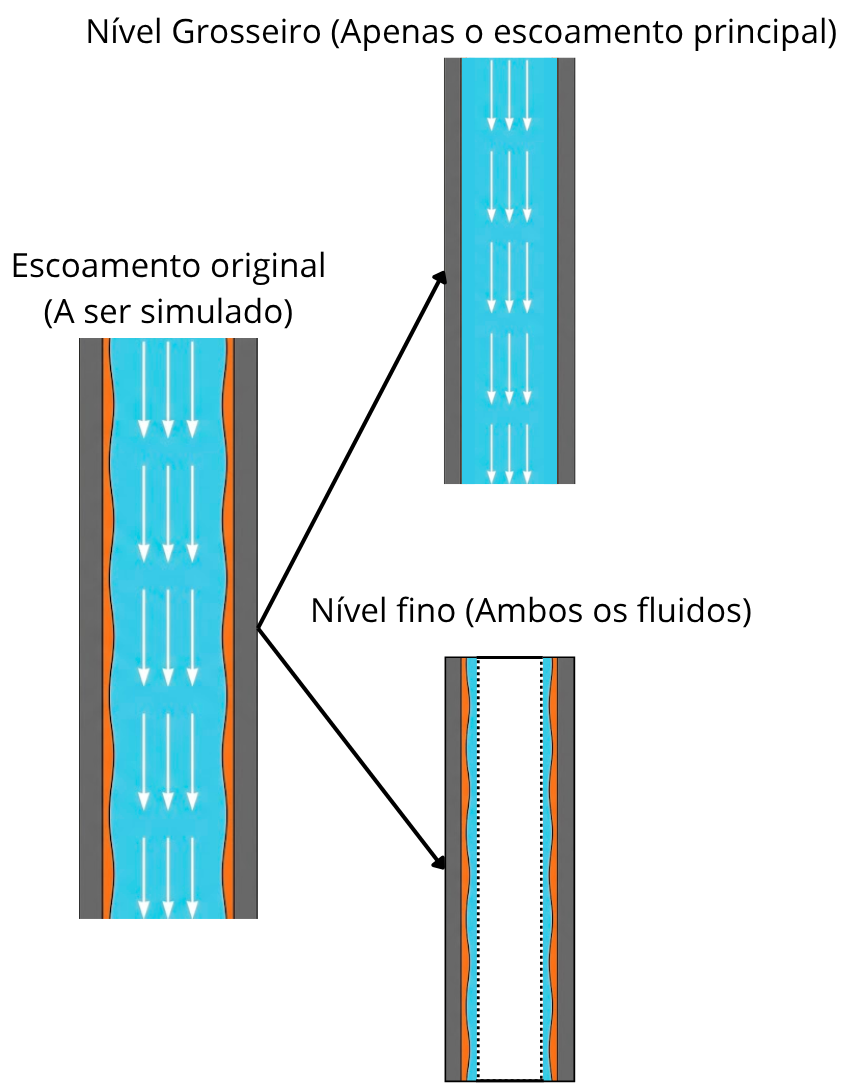
\includegraphics[width=0.8\textwidth]{imagens/completo_s_mesh.png}
    \caption{Divisão da simulação em domínios separados.}
    \label{fig:metodo-esquema}
\end{figure}

O acoplamento entre os domínios é bidirecional. O escoamento principal fornece ao filme as condições de contorno nos limites que que o domínio não encontra fronteira computacional e o filme devolve sua influência ao escoamento principal por meio da condição de contorno aplicada às paredes, sem que o escoamento principal precise enxergar a interface. As grandezas transferidas em cada via do acoplamento e as condições de contorno entre o filme e o core flow são tratados na Seção \ref{sec:acoplamento}. Os domínios também possuem seu próprio passo de tempo, que será tratado na Seção \ref{sec:passo-tempo}.

Dada a generalidade da proposta, o domínio $\Omega_f$ pode ser resolvido por
qualquer técnica clássica de escoamentos multifásicos, como modelos Euler-Euler, VOF
ou \textit{level-set}, desde que a técnica escolhida seja capaz de capturar a física
envolvida no processo e de fornecer informação sobre a posição e o estado da
interface, requisito imposto pelo acoplamento. Do escoamento principal exige-se que
seja resolvido de forma completa, com acoplamento pressão-velocidade, uma vez que é
dele que parte a informação de pressão para a banda. Em $\Omega_f$, por outro lado,
propõe-se eliminar o cálculo da correção da pressão, com o campo de pressão sendo
interpolado de $\Omega_p$, o que retira do domínio refinado a etapa mais cara da
solução.

A decomposição descrita se apoia nas seguintes hipóteses:

Para uma distinção, onde for cabível, adota-se ao longo deste capítulo fluido 1 como aquele que compõe o filme e fluido 2 como aquele que compõe o escoamento principal.

\begin{itemize}
    \item o fluido 1 permanece confinado em $\Omega_f$ ao longo de toda a simulação,
          de forma que $\Omega_p$ possa ser tratado como monofásico;
    \item não há estruturas da segunda fase fora da banda, ficando fora do escopo os
          regimes com entranhamento de gotas e com destacamento de porções do filme;
    \item os fluidos são incompressíveis, newtonianos e imiscíveis, com tensão
          superficial constante;
    \item o escoamento é isotérmico e laminar, sem mudança de fase e sem modelagem
          de turbulência.
\end{itemize}


\section{Particularização para o MFSim}

A descrição da Seção \ref{sec:visao-geral} não fixa a forma como os dois domínios são construídos nem como a informação transita entre eles. Na implementação adotada neste trabalho, ambos são obtidos da hierarquia de níveis de malha do \textit{MFSim} (citar artigos de MFSim), código de simulação fluidodinâmica desenvolvido no MFLab/UFU, que resolve as equações de balanço pelo método dos volumes finitos em malha deslocada. Aproveitar essa estrutura dispensa a construção de duas malhas independentes e de um procedimento de busca entre elas, uma vez que os operadores de interpolação entre níveis já existem no código.

\section{Sistema de Hierarquia de Níveis}

O  utilizado código possui uma estrutura hierárquica de níveis aninhados, que serve para fornecer estrutura aos algorítimos de refinamento de malha adaptativa (\textit{AMR}) e \textit{multigrid} (cite trabalhos). Essa hierarquia de níveis é mostrada na Figura \ref{fig:hierarquia_de_niveis}. Cada um dos níveis possui resíduos das variáveis calculadas pelo multigrid ou campos vetoriais completos quando esses níveis pertencerem aos níveis físicos do AMR.

\begin{figure}[H]
    \centering
    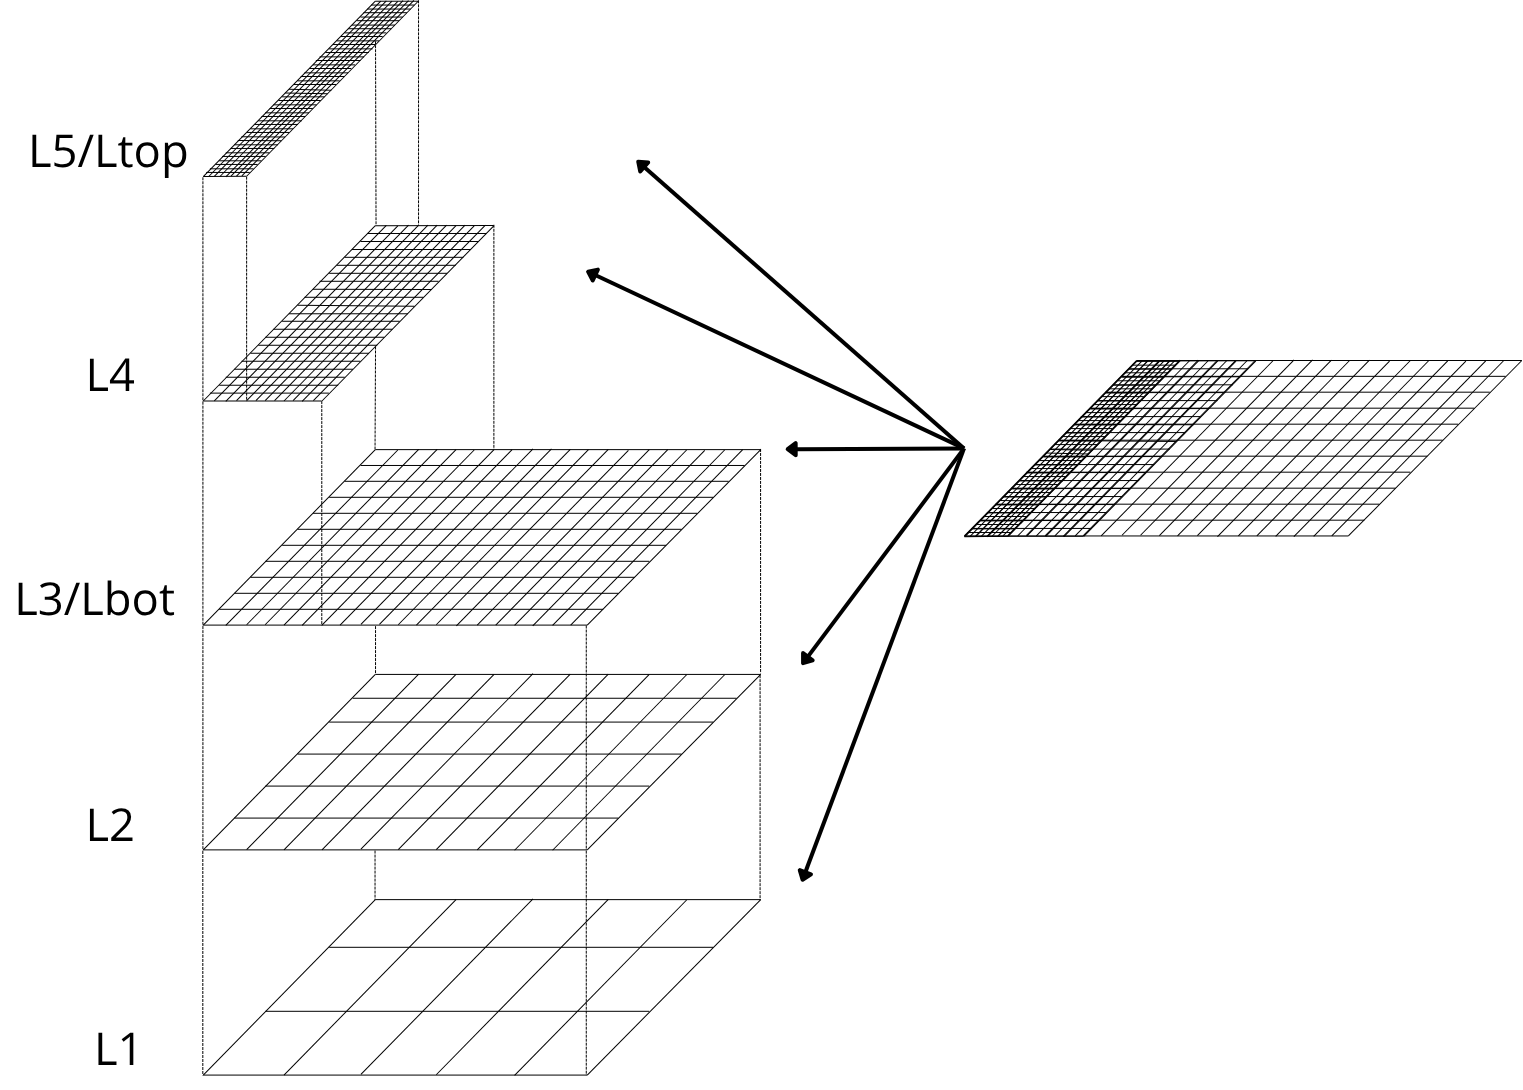
\includegraphics[width=0.7\textwidth]{imagens/estrutura_grid_mfsim.png}
    \caption{Esquema de como os níveis de malha se comportam no MFSim.}
    \label{fig:hierarquia_de_niveis}
\end{figure}

Tem-se então a divisão entre os níveis físicos, aqueles que resolvem o escoamento em si, os níveis intermediários que são apenas interpolados, e os níveis virtuais, que servem exclusivamente para a aplicação do método \textit{multigrid}. No exemplo da Figura \ref{fig:hierarquia_de_niveis} os níveis de L3 e L5 seriam os níveis físicos e os níveis L1 e L2 seriam apenas virtuais, tendo ainda o nível L4 que nesse contexto atuaria como nível intermediário.

Dessa forma, os níveis físicos guardam os campos, escalares e vetoriais, das propriedades físicas como: pressão, velocidade, e $f$ quando aplicável necessários para as interpolações do \textit{AMR} bem como os campos de resíduo e erro, necessários para a aplicação do \textit{multigrid}. Os níveis virtuais, porém, guardam apenas os campos resíduo e erro, sem terem informações dos campos vetoriais e escalares.


Dentro desta estrutura, os níveis físicos mais refinados resolvem suas condições de contorno a partir das condições globais, nas faces que encostam no limite do domínio, e a partir de interpolações de valores dos níveis inferiores nas faces que não tocam a fronteira do domínio.

Para o melhor entendimento da metodologia convenciona-se aqui \textit{ltop} o nível mais refinado da hierarquia multiníveis e como \textit{lbot} o último nível físico antes dos virtuais.

A metodologia proposta prevê confinar o escoamento bifásico no \textit{ltop}, assim sendo esse nível é "destacado" do ciclo de \textit{multigrid} e \textit{AMR} não sendo enxergado pelos demais, aos quais afeta de forma indireta. Nos níveis inferiores resolve-se o escoamento monofásico, sobre o qual são executados os ciclos e interpolações dos métodos mencionados sem a interferência do nível mais alto. Os níveis intermediários servem para guardar os campos, vindos dos níveis inferiores, para que sirvam de condição de contorno para o \textit{ltop}. A figura \ref{fig:hierarquia_metodo} mostra como a divisão funciona e o que roda em cada nível.

Os patches que pertencem ao \textit{ltop} estão sempre em contato, para pelo menos uma de suas faces, com a fronteira com o domínio ou com a fronteira imersa se utilizada e suas dimensões devem ser condizentes com a física esperada do filme, de forma que o fluido 1 esteja sempre confinado nos níveis mais finos da hierarquia. Apesar dos níveis inferiores não enxergarem diretamente o escoamento bifásico confinado, eles são influenciados pelo mesmo a partir das condições de contorno junto à parede que possui o filme.

\begin{figure}
    \centering
    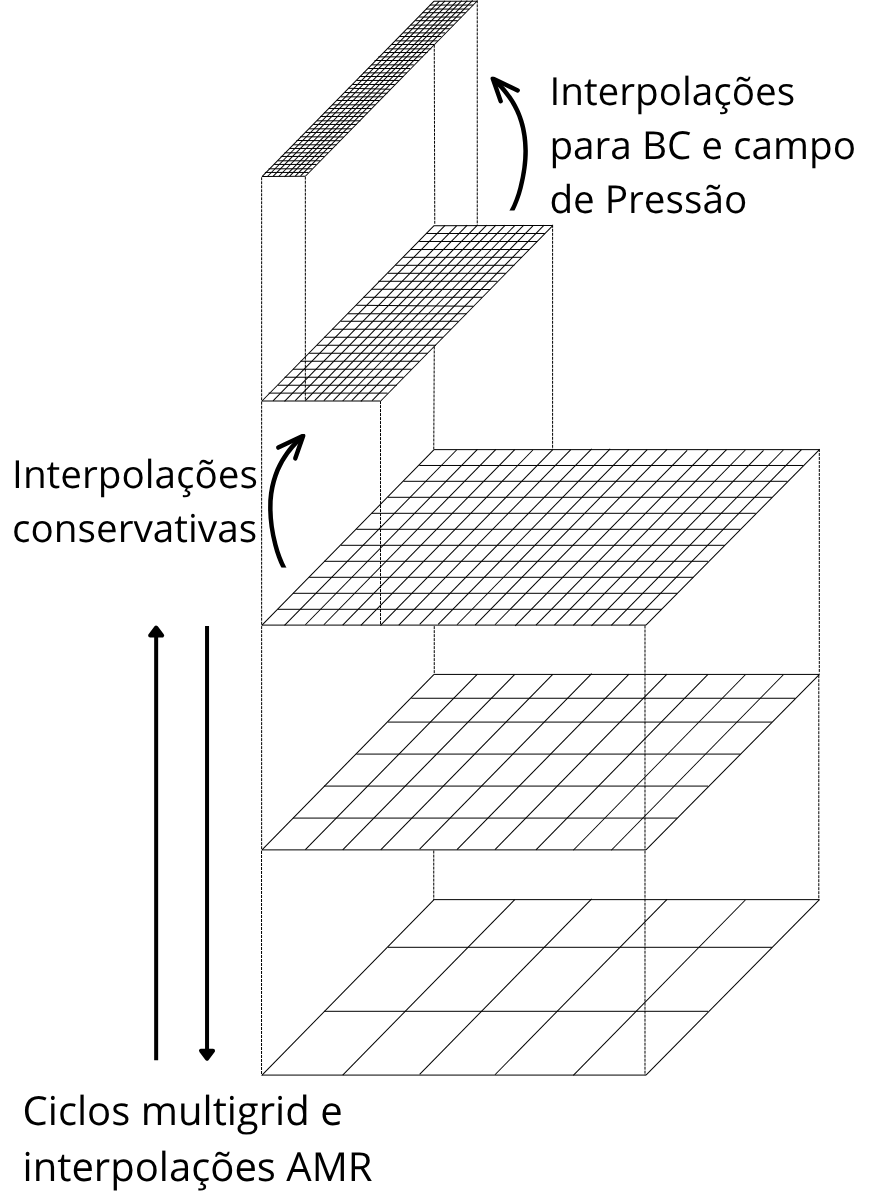
\includegraphics[width=0.7\textwidth]{imagens/hierarquia_de_interpolacoes.png}
    \caption{Esquema de como cada nível observa o outro e a direção na qual as interpolações são feitas.}
    \label{fig:hierarquia_metodo}
\end{figure}




\input{textual/Modelo-matematico.tex}


%=====================================================================
\input{textual/metodo/Escoamento_Principal}
%=====================================================================

